\documentclass[]{book}
\usepackage{lmodern}
\usepackage{amssymb,amsmath}
\usepackage{ifxetex,ifluatex}
\usepackage{fixltx2e} % provides \textsubscript
\ifnum 0\ifxetex 1\fi\ifluatex 1\fi=0 % if pdftex
  \usepackage[T1]{fontenc}
  \usepackage[utf8]{inputenc}
\else % if luatex or xelatex
  \ifxetex
    \usepackage{mathspec}
  \else
    \usepackage{fontspec}
  \fi
  \defaultfontfeatures{Ligatures=TeX,Scale=MatchLowercase}
\fi
% use upquote if available, for straight quotes in verbatim environments
\IfFileExists{upquote.sty}{\usepackage{upquote}}{}
% use microtype if available
\IfFileExists{microtype.sty}{%
\usepackage{microtype}
\UseMicrotypeSet[protrusion]{basicmath} % disable protrusion for tt fonts
}{}
\usepackage[margin=1in]{geometry}
\usepackage{hyperref}
\hypersetup{unicode=true,
            pdftitle={Introduction to Machine Learning},
            pdfauthor={JJ Valletta},
            pdfborder={0 0 0},
            breaklinks=true}
\urlstyle{same}  % don't use monospace font for urls
\usepackage{longtable,booktabs}
\usepackage{graphicx,grffile}
\makeatletter
\def\maxwidth{\ifdim\Gin@nat@width>\linewidth\linewidth\else\Gin@nat@width\fi}
\def\maxheight{\ifdim\Gin@nat@height>\textheight\textheight\else\Gin@nat@height\fi}
\makeatother
% Scale images if necessary, so that they will not overflow the page
% margins by default, and it is still possible to overwrite the defaults
% using explicit options in \includegraphics[width, height, ...]{}
\setkeys{Gin}{width=\maxwidth,height=\maxheight,keepaspectratio}
\IfFileExists{parskip.sty}{%
\usepackage{parskip}
}{% else
\setlength{\parindent}{0pt}
\setlength{\parskip}{6pt plus 2pt minus 1pt}
}
\setlength{\emergencystretch}{3em}  % prevent overfull lines
\providecommand{\tightlist}{%
  \setlength{\itemsep}{0pt}\setlength{\parskip}{0pt}}
\setcounter{secnumdepth}{5}
% Redefines (sub)paragraphs to behave more like sections
\ifx\paragraph\undefined\else
\let\oldparagraph\paragraph
\renewcommand{\paragraph}[1]{\oldparagraph{#1}\mbox{}}
\fi
\ifx\subparagraph\undefined\else
\let\oldsubparagraph\subparagraph
\renewcommand{\subparagraph}[1]{\oldsubparagraph{#1}\mbox{}}
\fi

%%% Use protect on footnotes to avoid problems with footnotes in titles
\let\rmarkdownfootnote\footnote%
\def\footnote{\protect\rmarkdownfootnote}

%%% Change title format to be more compact
\usepackage{titling}

% Create subtitle command for use in maketitle
\newcommand{\subtitle}[1]{
  \posttitle{
    \begin{center}\large#1\end{center}
    }
}

\setlength{\droptitle}{-2em}

  \title{Introduction to Machine Learning}
    \pretitle{\vspace{\droptitle}\centering\huge}
  \posttitle{\par}
    \author{\href{mailto:jj.valletta@exeter.ac.uk}{JJ Valletta}}
    \preauthor{\centering\large\emph}
  \postauthor{\par}
      \predate{\centering\large\emph}
  \postdate{\par}
    \date{16 March 2019}

% latex macro to create task boxes
\usepackage{tcolorbox, comment}
\tcbuselibrary{breakable}

\definecolor{taskCol}{HTML}{404040}
\definecolor{taskCol1}{HTML}{808080}

\tcbset{colback=white,colframe=taskCol,arc=0mm}

%trick to fool markdown into compiling
\newcommand{\bblockT}[2][Task]{\begin{tcolorbox}[title = #1 #2, parbox = false]}
\newcommand{\eblockT}{\end{tcolorbox}}
\newcommand{\bblockS}[2][Solution]{\begin{tcolorbox}[title = #1 #2, colframe=taskCol1, breakable, parbox = false]}
\newcommand{\eblockS}{\end{tcolorbox}}

%add tabbed solutions environment
\newcommand{\bmp}{\begin{minipage}[c]{0.5\textwidth}}
\newcommand{\emp}{\end{minipage}}
\newcommand{\bblockST}[1]{\begin{tcolorbox}[title = #1, colframe=taskCol1, breakable, parbox = false]}
\newcommand{\eblockST}{\end{tcolorbox}}

%set solution button link
\usepackage{tikz}

\newcommand{\buttonT}[1]{
    \begin{tikzpicture}
    \node[
        inner sep=5pt,
        draw=taskCol,
        fill=taskCol,
        rounded corners=2pt,
        text=white
    ] (c1) {#1};
    \end{tikzpicture}
}

\newcommand{\buttonS}[1]{
    \begin{tikzpicture}
    \node[
        inner sep=5pt,
        draw=taskCol1,
        fill=taskCol1,
        rounded corners=2pt,
        text=white
    ] (c1) {#1};
    \end{tikzpicture}
}

\newcommand{\colpageref}[1]{\hypersetup{linkcolor=white}\pageref{#1}}

\begin{document}
\maketitle

{
\setcounter{tocdepth}{1}
\tableofcontents
}
\hypertarget{preface}{%
\chapter*{Preface}\label{preface}}
\addcontentsline{toc}{chapter}{Preface}

An introductory workshop on the field of machine learning. The focus will be on how to use these methods
in practice using R and Python, rather than on the rigorous underlying mathematics. The target audience
is anyone who wants to know what machine learning is, what problems it can solve and how we solve them
in practice using R and Python.

\hypertarget{prerequisites}{%
\section*{Prerequisites}\label{prerequisites}}
\addcontentsline{toc}{section}{Prerequisites}

\begin{itemize}
\tightlist
\item
  Programming basics in either R or Python
\end{itemize}

\hypertarget{learning-outcomes}{%
\section*{Learning outcomes}\label{learning-outcomes}}
\addcontentsline{toc}{section}{Learning outcomes}

\begin{itemize}
\tightlist
\item
  Understand the key concepts and terminology used in the field of machine learning
\item
  Build predictive models for clustering, regression and classification problems
\item
  Apply machine learning algorithms in R/Python to a variety of real-world datasets
\item
  Recognise practical issues in data-driven modelling
\end{itemize}

\hypertarget{recommended-reading}{%
\section*{Recommended reading}\label{recommended-reading}}
\addcontentsline{toc}{section}{Recommended reading}

I highly recommend the following books:

\begin{itemize}
\tightlist
\item
  \href{http://www-bcf.usc.edu/~gareth/ISL/}{An Introduction to Statistical Learning}
\item
  \href{https://web.stanford.edu/~hastie/ElemStatLearn/}{The Elements of Statistical Learning}
\item
  \href{https://www.springer.com/gp/book/9780387310732}{Pattern Recognition and Machine Learning}
\item
  \href{https://www.cs.ubc.ca/~murphyk/MLbook/}{Machine Learning: A Probabilistic Perspective}
\end{itemize}

\hypertarget{software-packages}{%
\section*{Software packages}\label{software-packages}}
\addcontentsline{toc}{section}{Software packages}

\begin{itemize}
\tightlist
\item
  R: \href{http://topepo.github.io/caret/index.html}{\texttt{caret}}
\item
  Python: \href{https://scikit-learn.org/stable/}{\texttt{scikit-learn}}
\end{itemize}

\hypertarget{data-files}{%
\section*{Data files}\label{data-files}}
\addcontentsline{toc}{section}{Data files}

All data files can be downloaded as a ZIP file from \href{https://exeter-data-analytics.github.io/StatModelling/dataFiles.zip}{here}.

\hypertarget{introduction}{%
\chapter{Introduction}\label{introduction}}

\hypertarget{motivation}{%
\section{Motivation}\label{motivation}}

\begin{itemize}
\tightlist
\item
  Scientists are nowadays faced with an unprecedented amount of complex and big data sets
  (e.g.~high-throughput sequencing, GIS (Geographical Information System) data, biomedical imaging and social media data).
\item
  These data sets are very challenging to analyse due to nonlinear dependencies, mixed data sources and high-dimensionality.
\item
  They often fail to conform to the assumptions of classical statistical methods.
\item
  Hand-in-hand with the rise of computational power, machine learning (ML), has matured into a field of its own,
  to specificially extract knowledge from these data.
\end{itemize}

\hypertarget{what-is-machine-learning}{%
\section{What is machine learning?}\label{what-is-machine-learning}}

\begin{quote}
A machine (an algorithm/model) improves its performance (predictive accuracy) in achieving a task (e.g
classifying the content of an image) from experience (data).
\end{quote}

\begin{quote}
The automatic discovery of patterns and regularities in data.
\end{quote}

\hypertarget{what-problems-can-machine-learning-solve}{%
\section{What problems can machine learning solve?}\label{what-problems-can-machine-learning-solve}}

\begin{itemize}
\item
  Object recognition
\item
  Biomarker discovery in genomics
\item
  Navigation of autonomous vehicles
\item
  Fraud detection
\item
  \ldots{} and much more!
\end{itemize}

\hypertarget{types-of-machine-learning-methods}{%
\section{Types of machine learning methods}\label{types-of-machine-learning-methods}}

\hypertarget{unsupervised-learning}{%
\subsection*{Unsupervised learning}\label{unsupervised-learning}}
\addcontentsline{toc}{subsection}{Unsupervised learning}

Unsupervised learning methods uncover structure in unlabelled data. Structure means patterns in the data that are sufficiently different from pure unstructured noise. Structure can be discovered by:

\begin{itemize}
\tightlist
\item
  Determining the distribution of the data using \textbf{density estimation} techniques
\end{itemize}

\begin{center}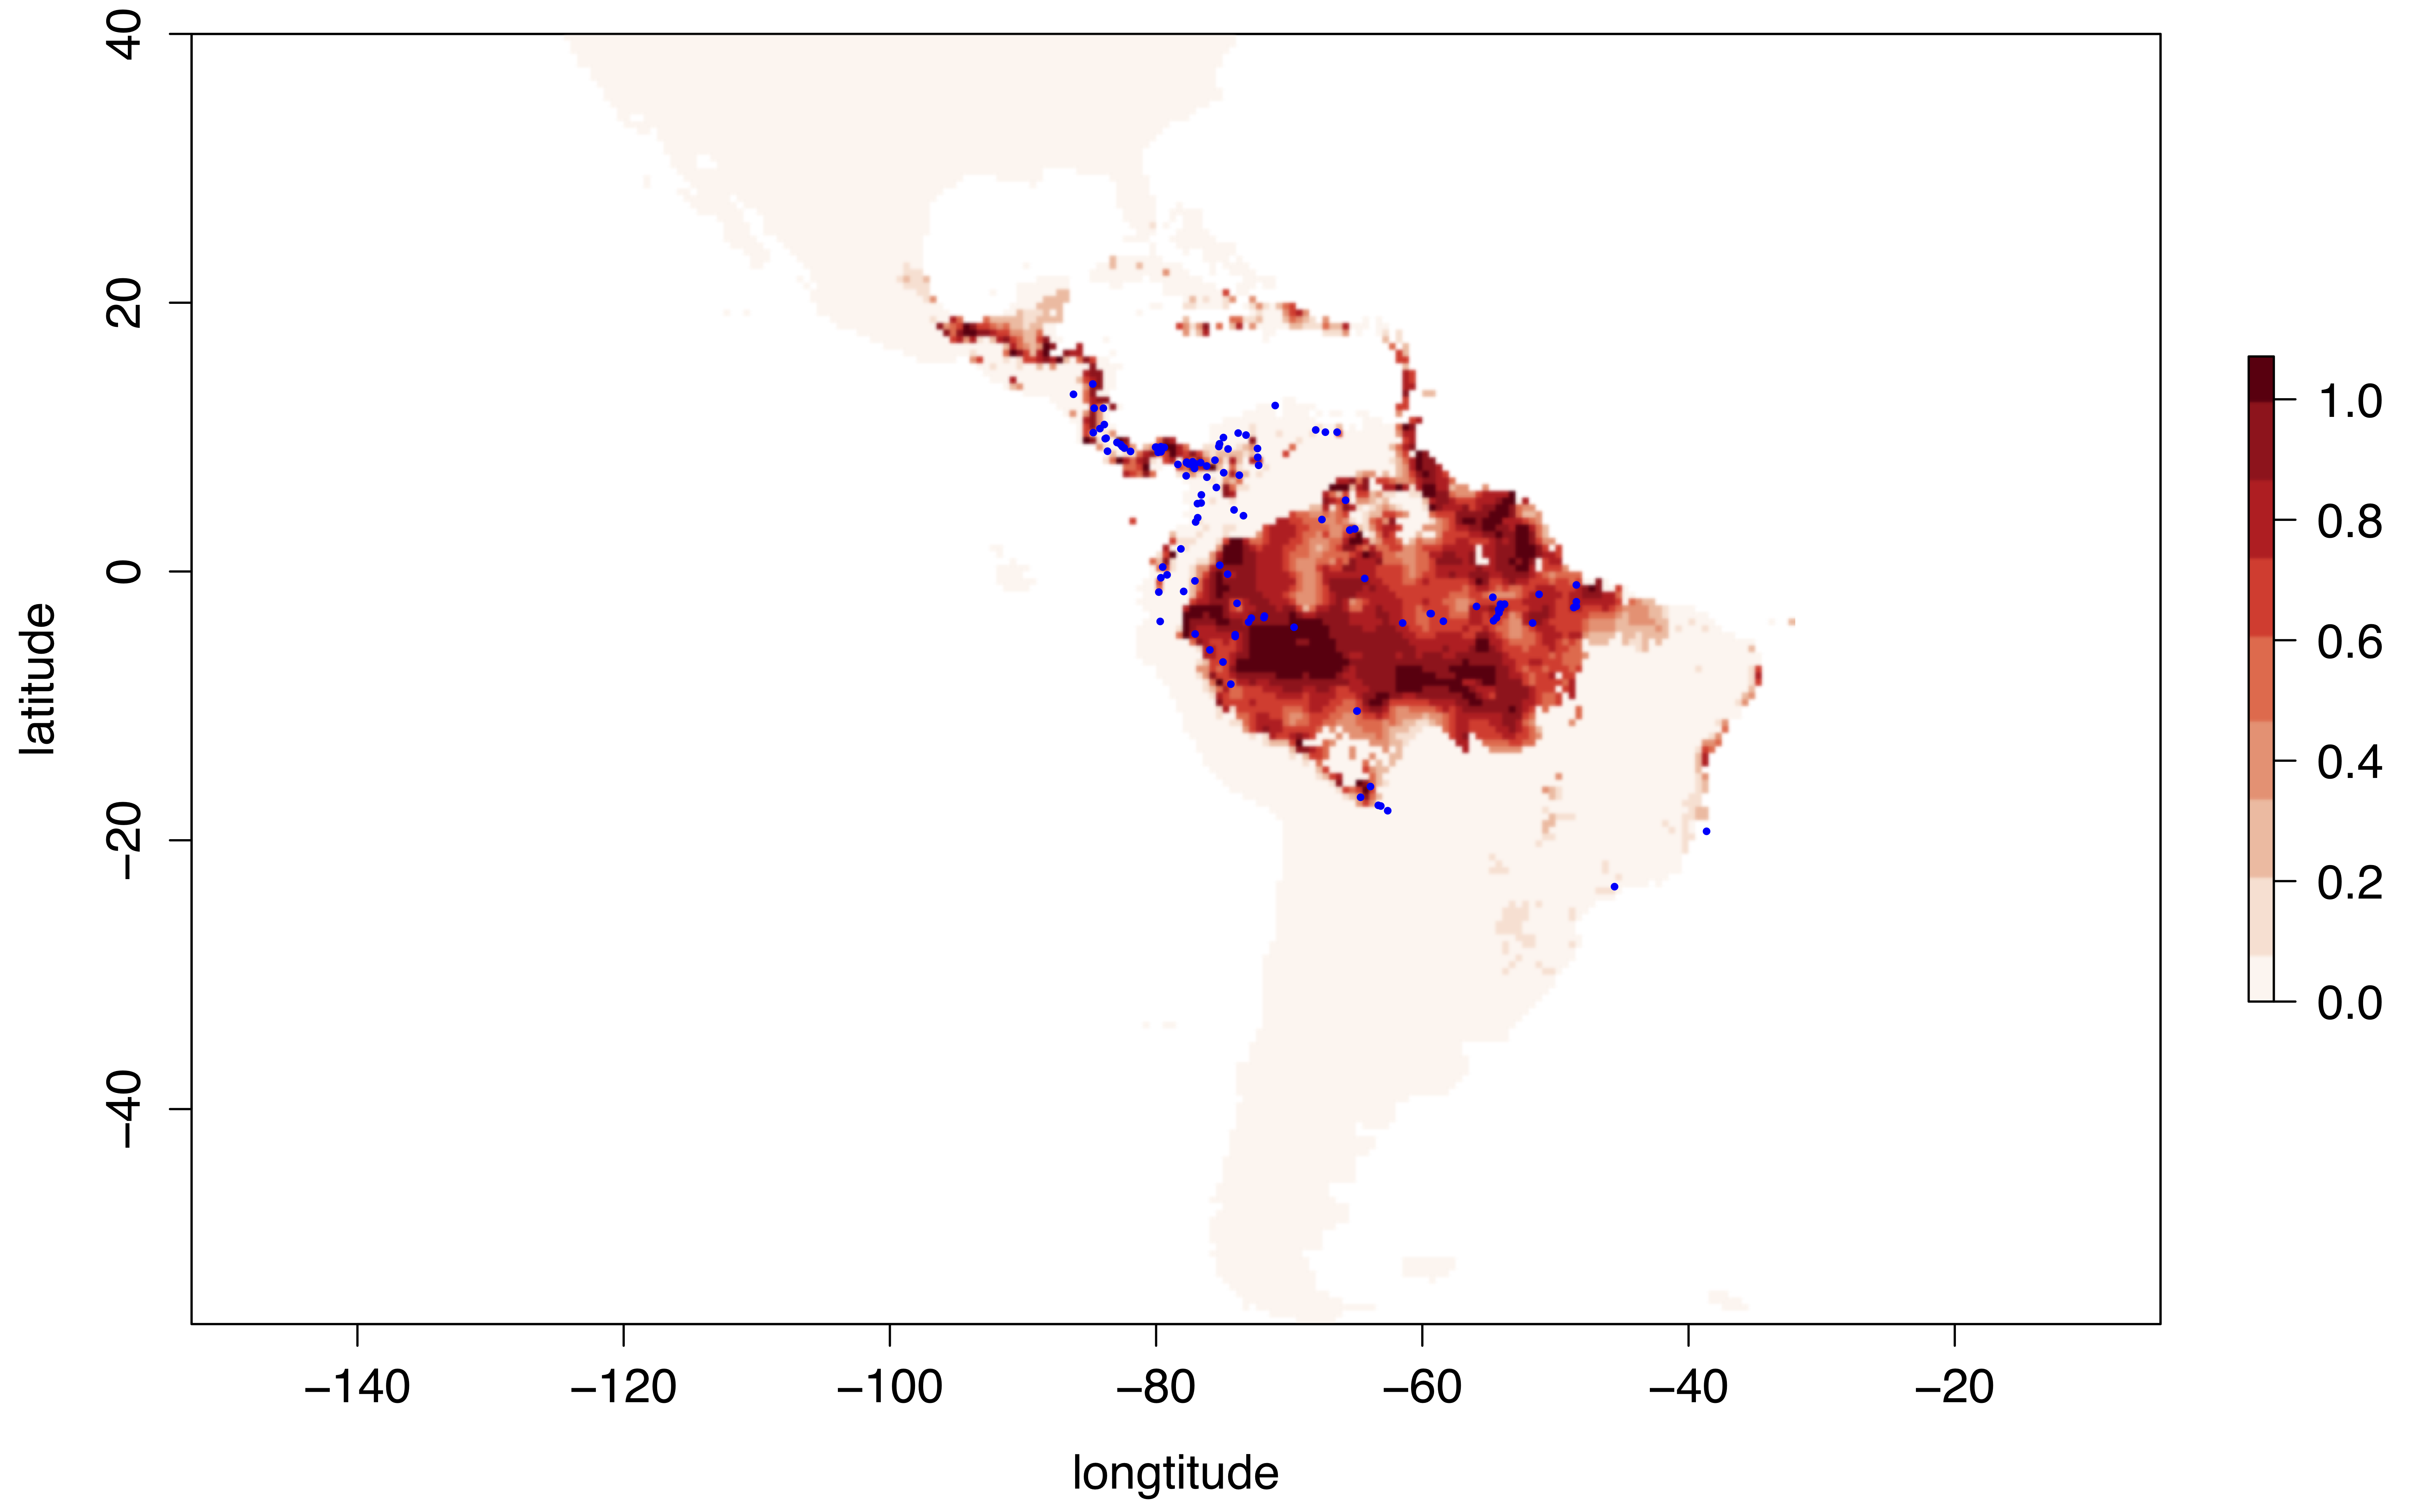
\includegraphics[width=600px]{_img//01-density} \end{center}

\begin{itemize}
\tightlist
\item
  Visualising the data after \textbf{dimensionality reduction} (e.g Principal Component Analysis (PCA))
\end{itemize}

\begin{center}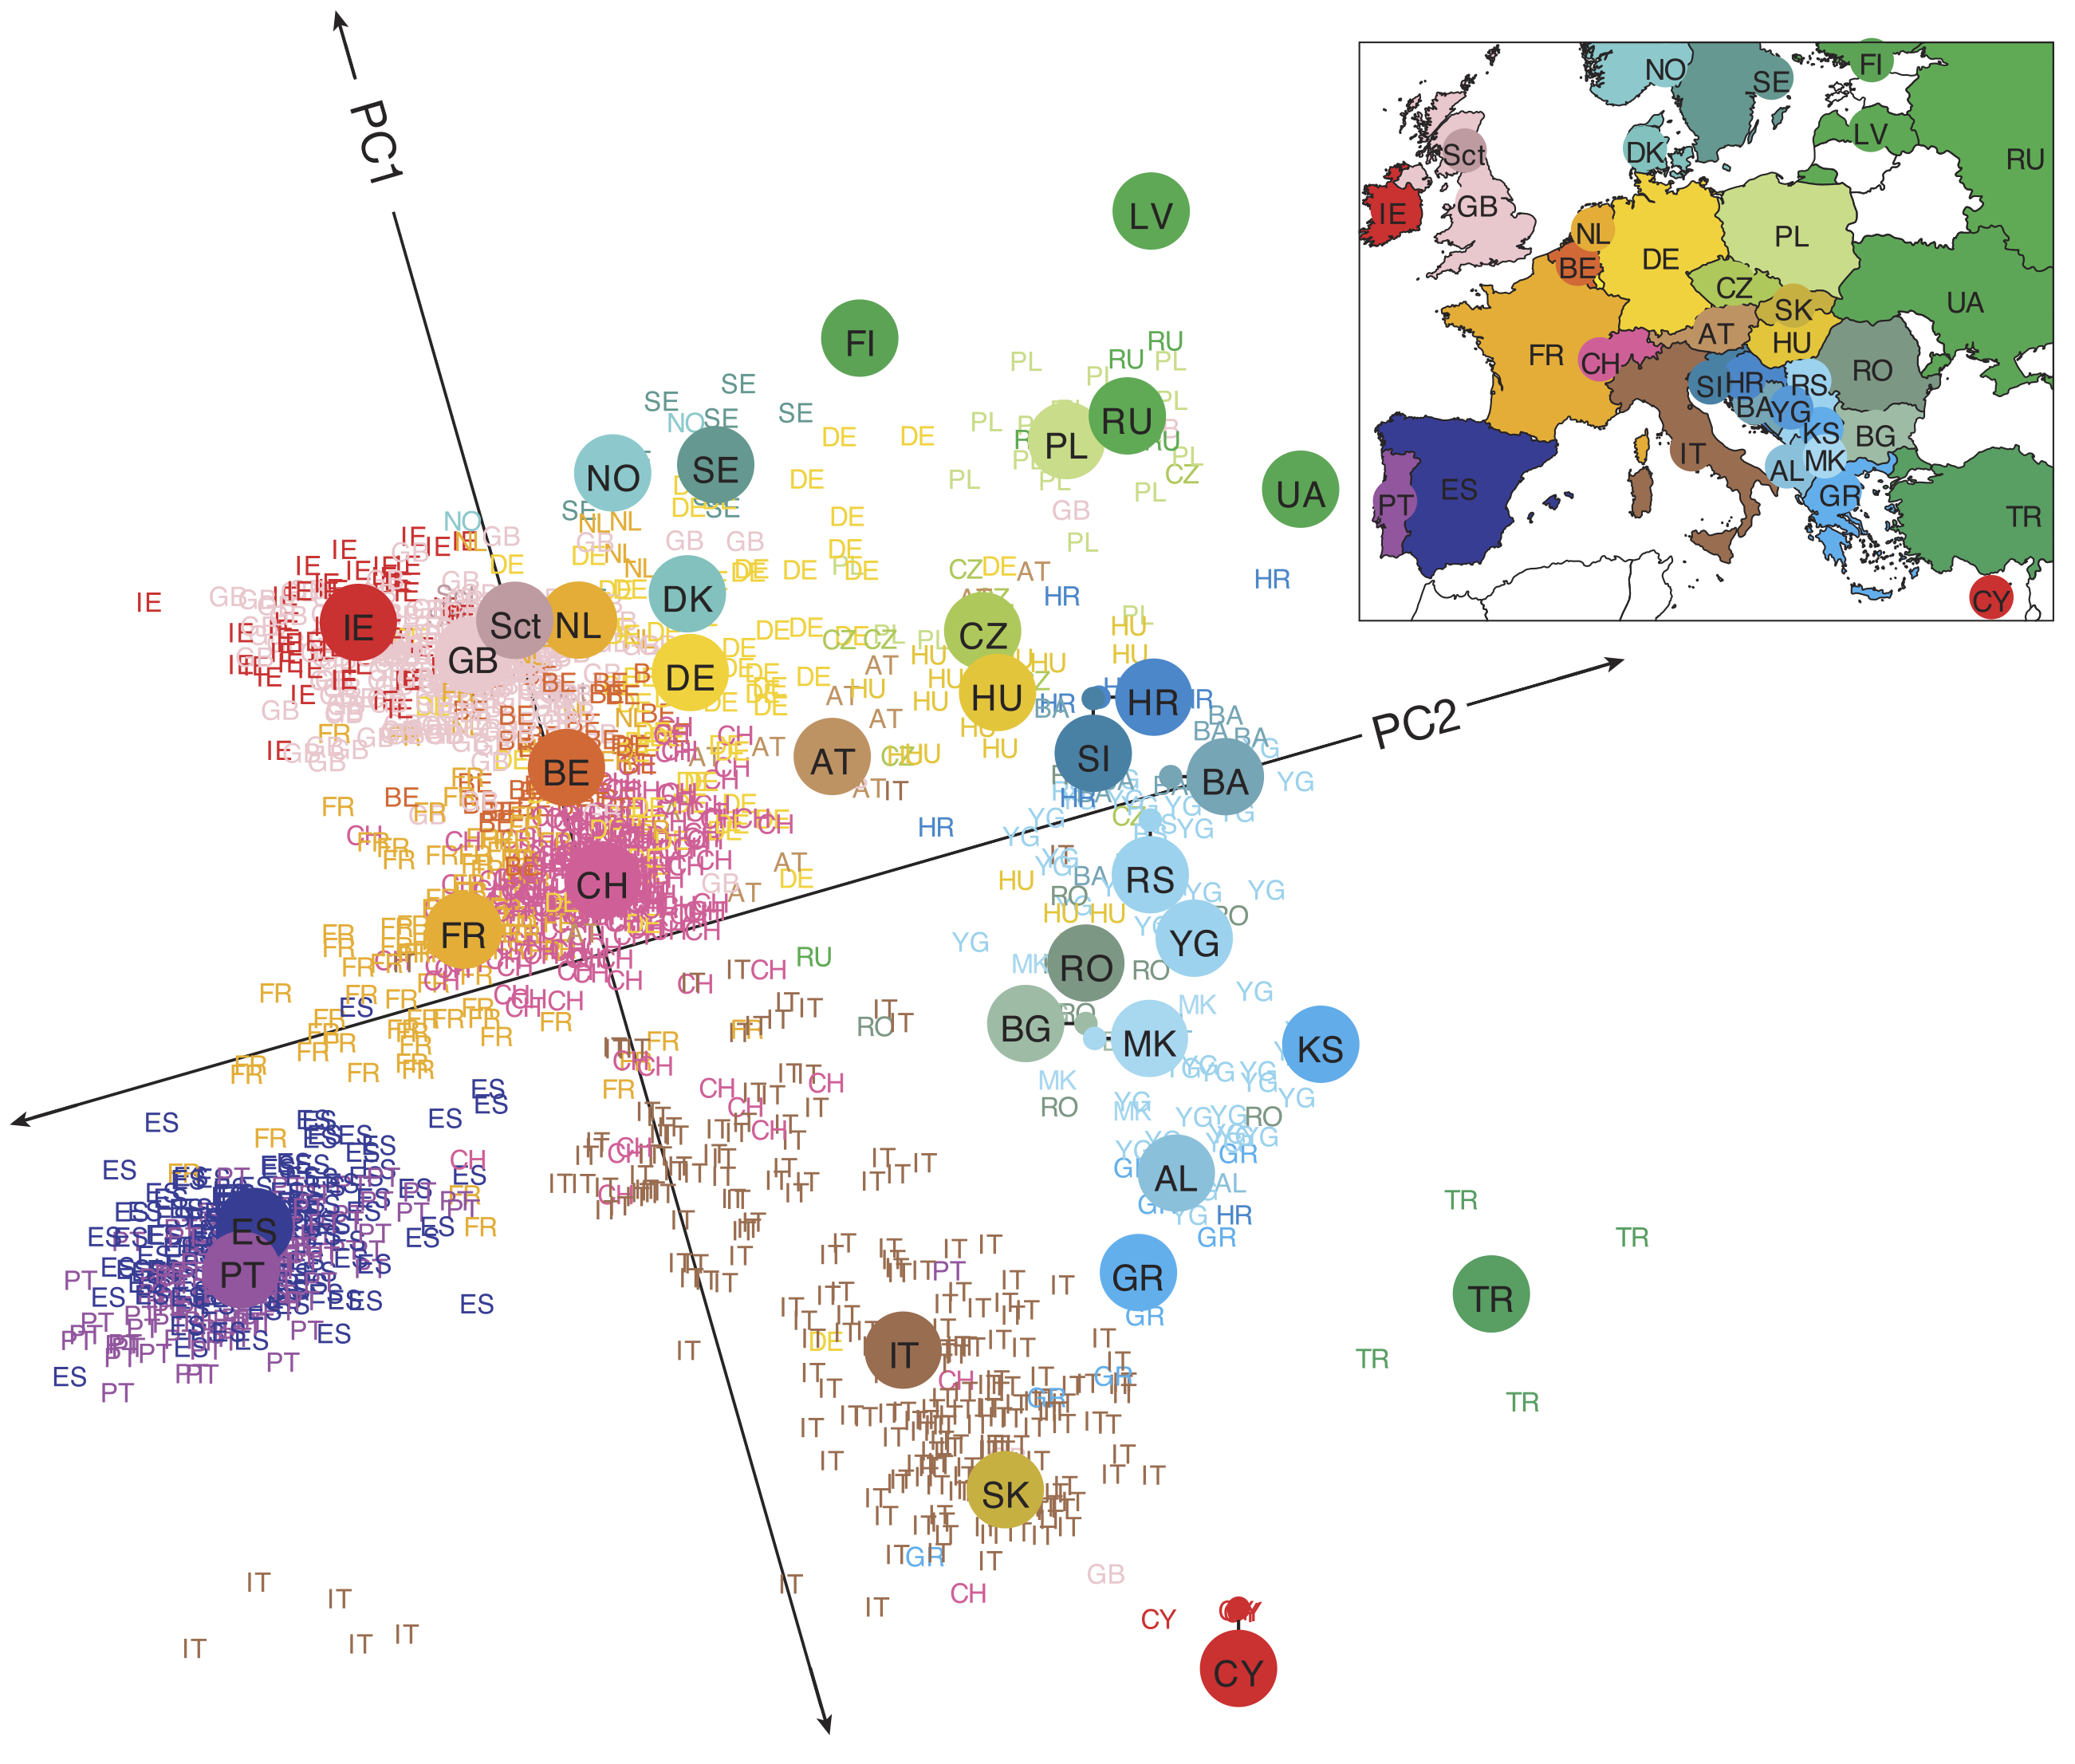
\includegraphics[width=600px]{_img//01-dimensionality} \end{center}

\begin{itemize}
\tightlist
\item
  Identifying groups of observations sharing similar attributes using \textbf{clustering} methods
\end{itemize}

\begin{center}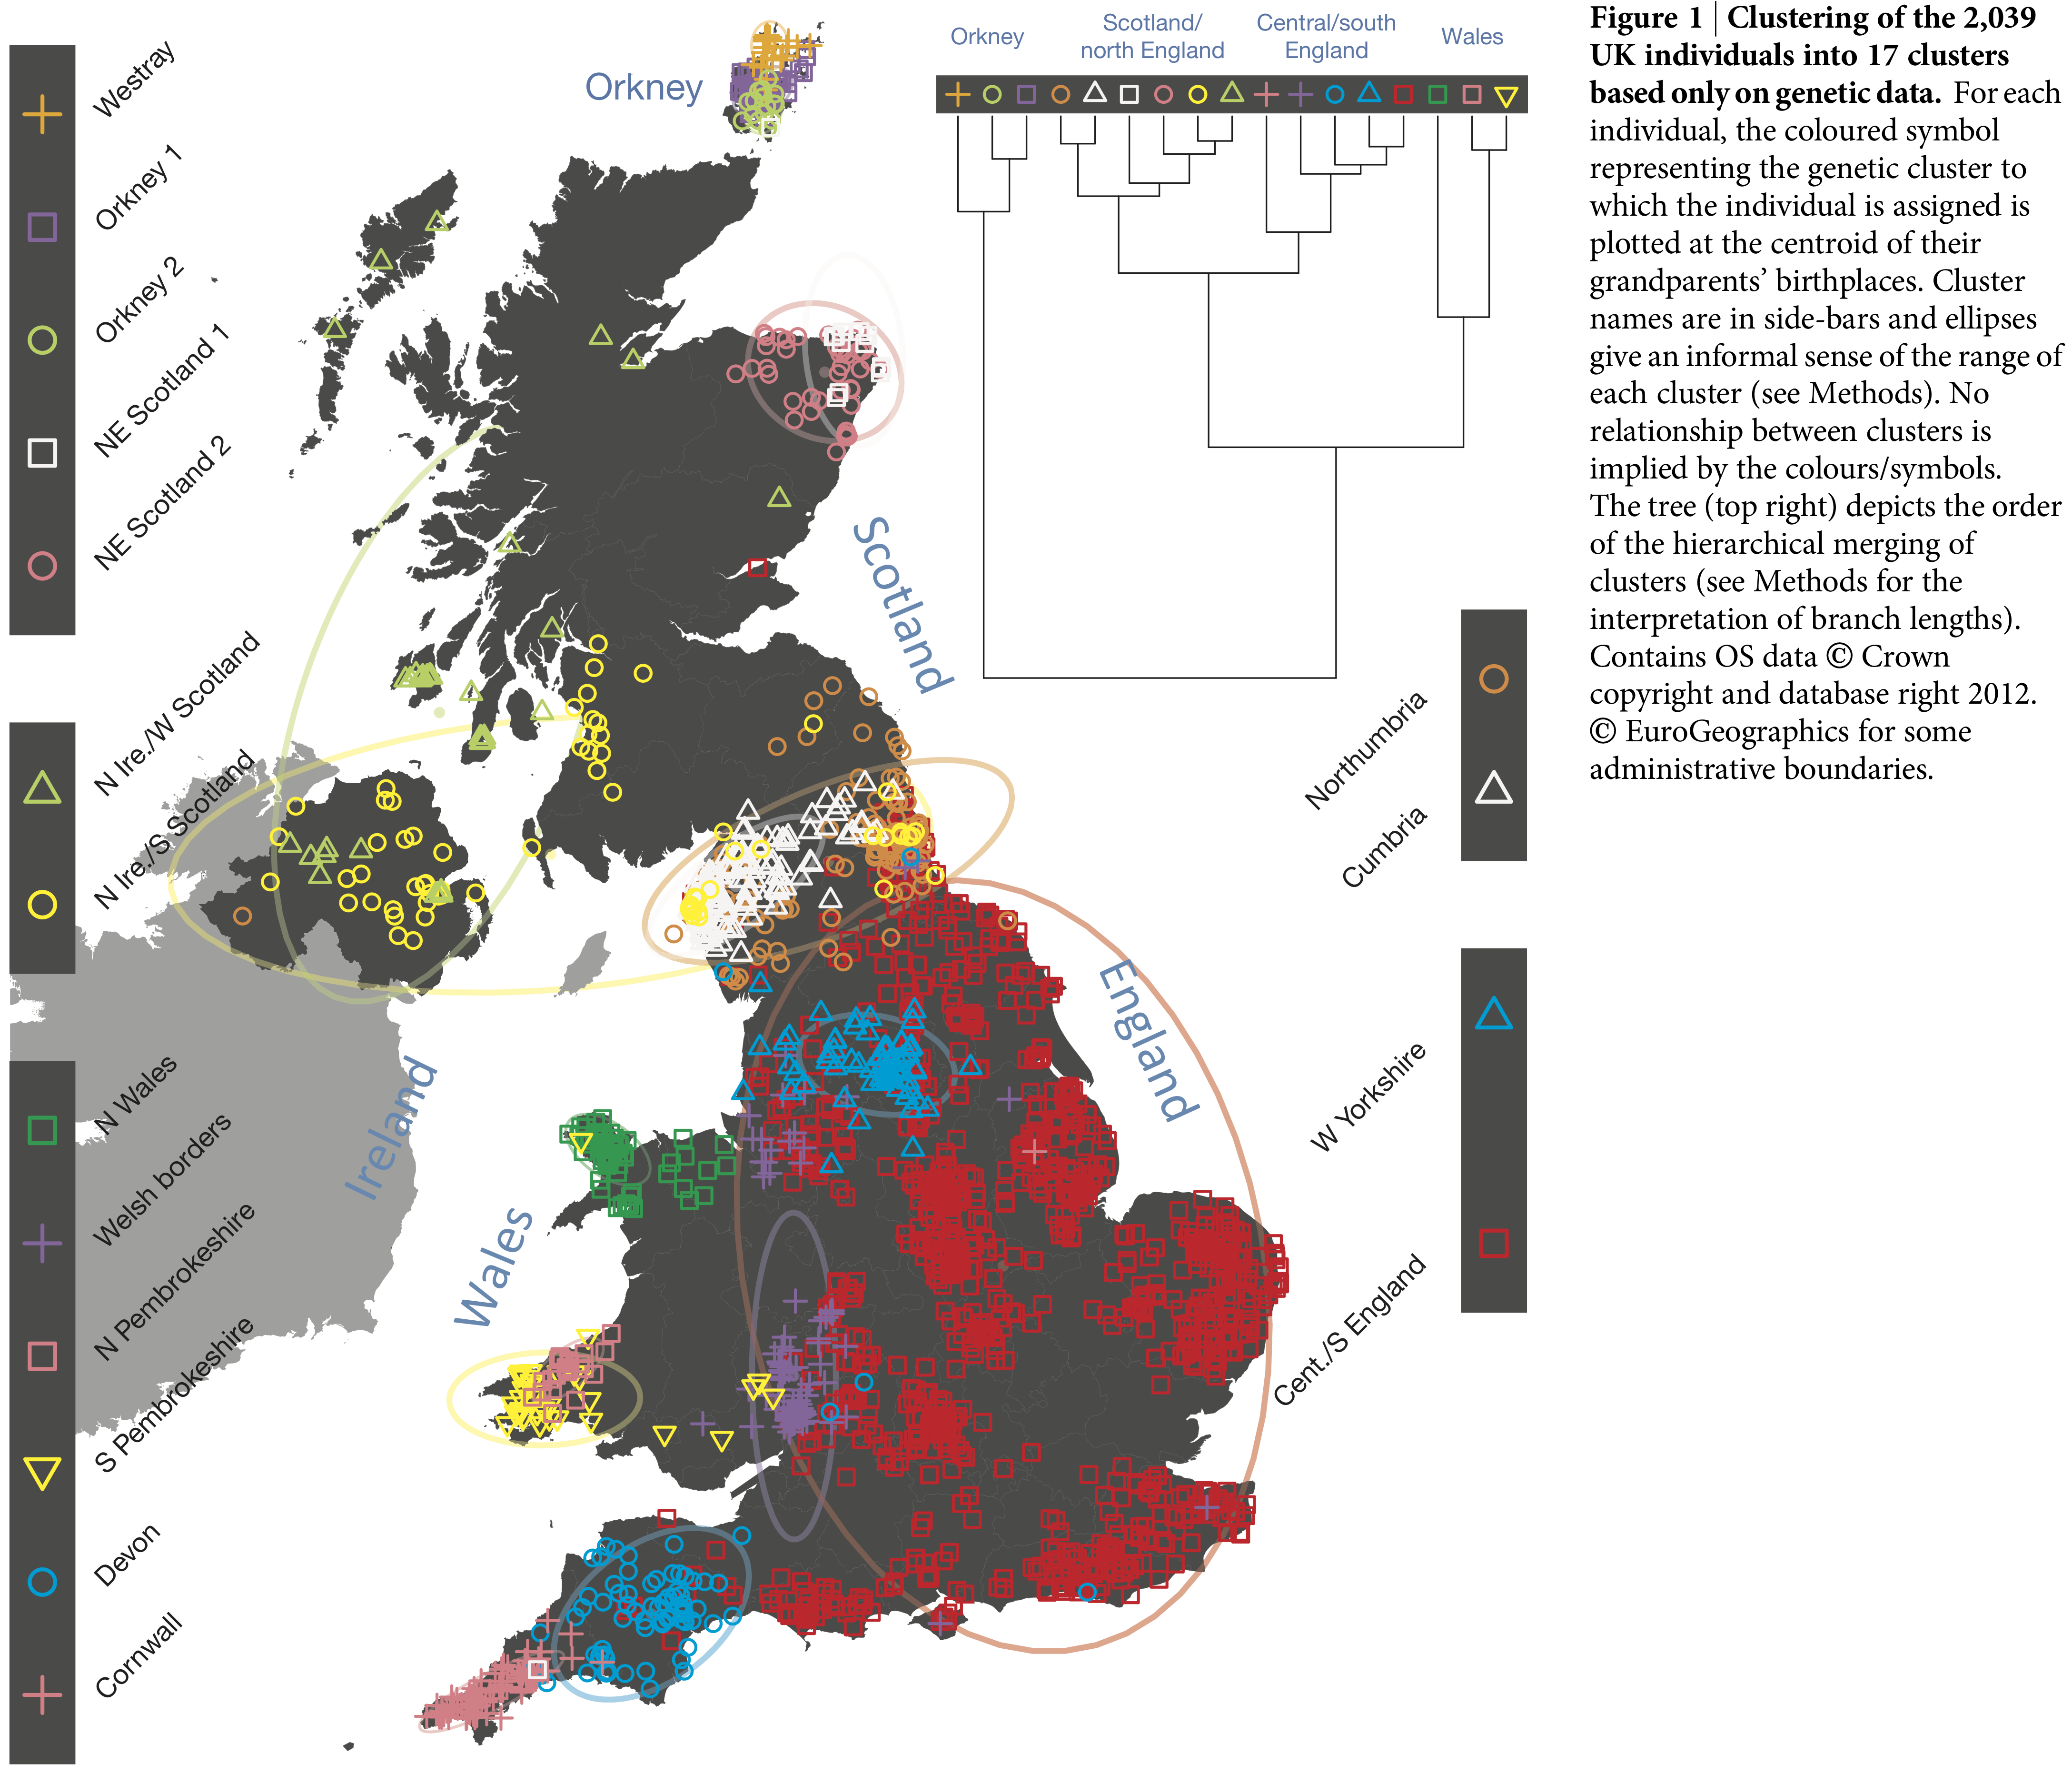
\includegraphics[width=600px]{_img//01-clustering} \end{center}

\hypertarget{supervised-learning}{%
\subsection*{Supervised learning}\label{supervised-learning}}
\addcontentsline{toc}{subsection}{Supervised learning}

Akin to traditional statistical models (e.g generalised linear models) supervised learning methods
discover the relationship between an outcome and a set of explanatory variables.
Using \textbf{training data}, the model learns the mapping (predictive model) between a set of features
and a:

\begin{itemize}
\tightlist
\item
  Continuous outcome - \textbf{regression}
\end{itemize}

\begin{center}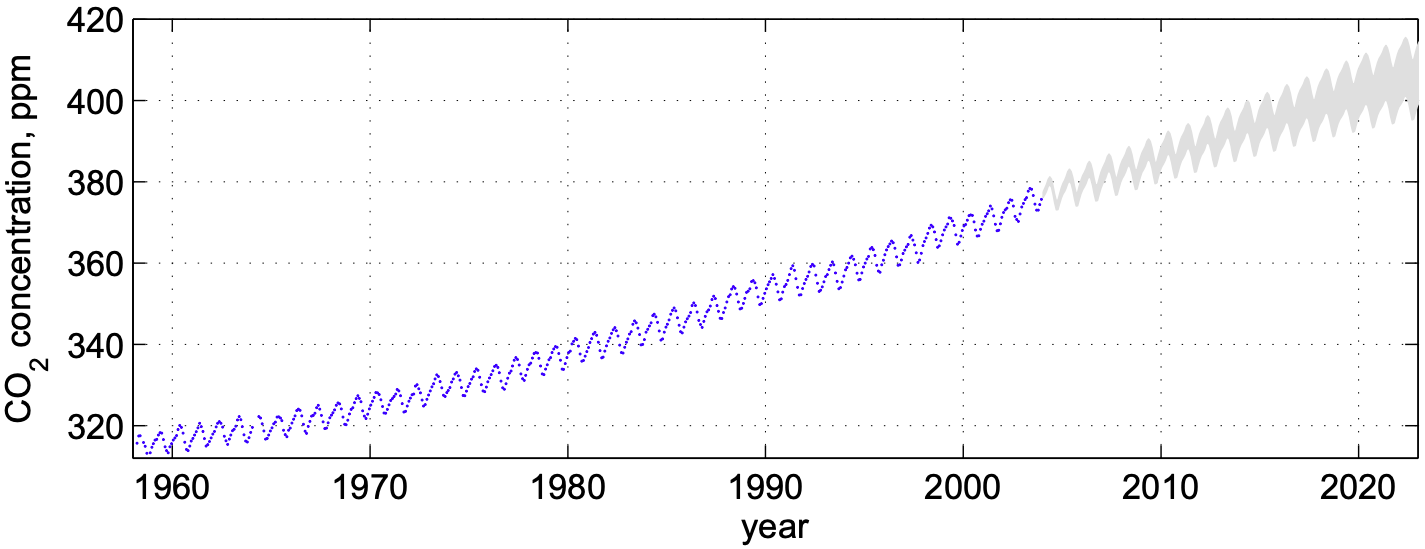
\includegraphics[width=600px]{_img//01-regression} \end{center}

\begin{itemize}
\tightlist
\item
  Categorical variable - \textbf{classification}
\end{itemize}

\begin{center}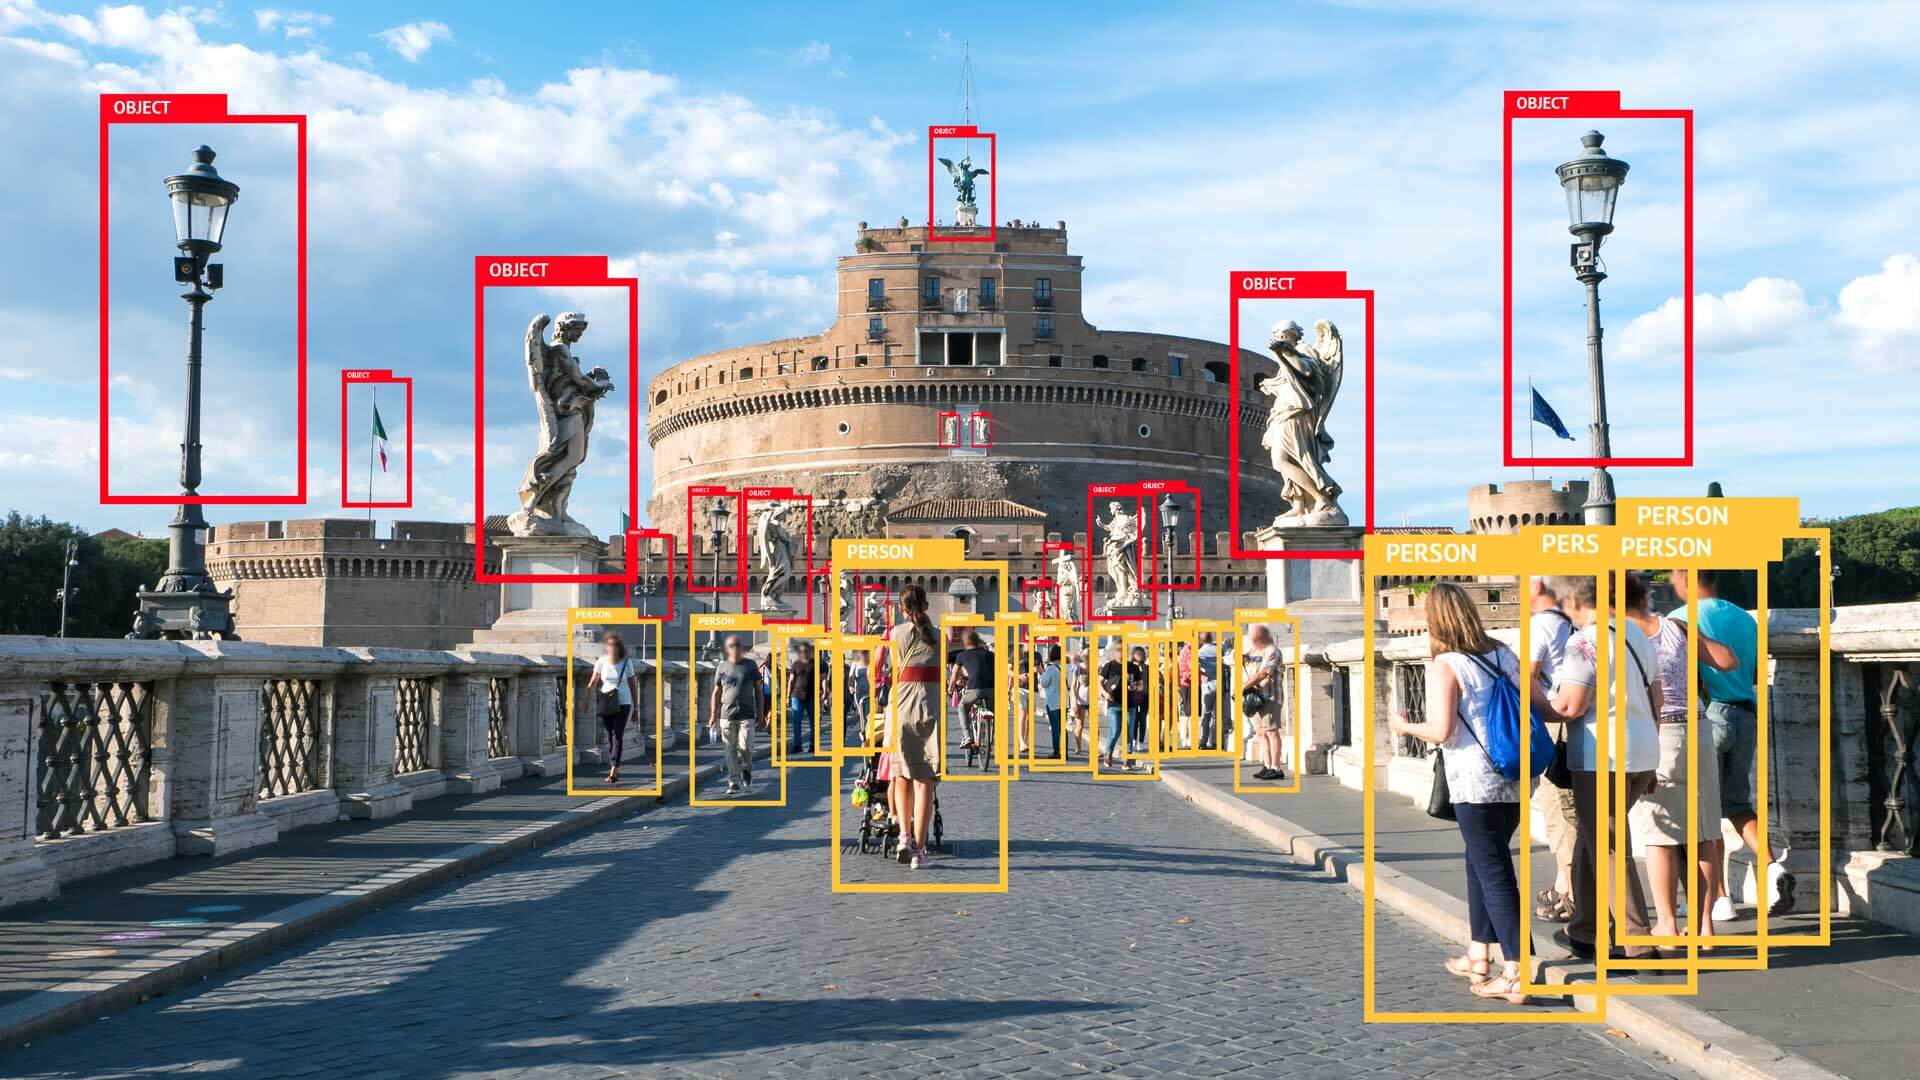
\includegraphics[width=600px]{_img//01-classification} \end{center}

\hypertarget{semi-supervised-learning}{%
\subsection*{Semi-supervised learning}\label{semi-supervised-learning}}
\addcontentsline{toc}{subsection}{Semi-supervised learning}

Similar to supervised learning, however these methods also make use of unlabelled data to improve
the model's predictive performance.

\hypertarget{reinforcement-learning}{%
\subsection*{Reinforcement learning}\label{reinforcement-learning}}
\addcontentsline{toc}{subsection}{Reinforcement learning}

These methods mimic the way humans learn new games or skills (e.g riding a unicycle).
The machine/model explores different actions that maximise a \textbf{reward} (e.g score achieved in a game or
time spent upright on a unicyle) by a process of trial and error.
There is an inherent tradeoff between \textbf{exploration} (trying out new actions) and
\textbf{exploitation} (use actions that already give reasonable results).

In this introductory workshop we will only focus on unsupervised and supervised learning methods.

\hypertarget{statistics-and-machine-learning}{%
\section{Statistics and Machine Learning}\label{statistics-and-machine-learning}}

There is substantial overlap between the fields of statistics and machine learning.
Some high-profile academics, such as Robert Tibshirani, even argue that ML is merely
``glorified statistics''. He also provides a handy \href{http://statweb.stanford.edu/~tibs/stat315a/glossary.pdf}{glossary}.

We will not enter into a philosophical debate here, rather we focus
on a pragmatic comparison between these two schools of thought,
which evolved from different research areas and tackled different problems.

\begin{longtable}[]{@{}lll@{}}
\toprule
\begin{minipage}[b]{0.10\columnwidth}\raggedright
\strut
\end{minipage} & \begin{minipage}[b]{0.41\columnwidth}\raggedright
Statistics\strut
\end{minipage} & \begin{minipage}[b]{0.41\columnwidth}\raggedright
Machine learning\strut
\end{minipage}\tabularnewline
\midrule
\endhead
\begin{minipage}[t]{0.10\columnwidth}\raggedright
\textbf{Philosophy}\strut
\end{minipage} & \begin{minipage}[t]{0.41\columnwidth}\raggedright
provide humans with a set of data analysis tools\strut
\end{minipage} & \begin{minipage}[t]{0.41\columnwidth}\raggedright
replace humans in the processing of data\strut
\end{minipage}\tabularnewline
\begin{minipage}[t]{0.10\columnwidth}\raggedright
\textbf{Focus}\strut
\end{minipage} & \begin{minipage}[t]{0.41\columnwidth}\raggedright
what is the relationship between the data and the outcome?\strut
\end{minipage} & \begin{minipage}[t]{0.41\columnwidth}\raggedright
how can we predict the outcome using the data?\strut
\end{minipage}\tabularnewline
\begin{minipage}[t]{0.10\columnwidth}\raggedright
\textbf{Inference}\strut
\end{minipage} & \begin{minipage}[t]{0.41\columnwidth}\raggedright
how was the observed data generated? what do the model parameters mean in practice?\strut
\end{minipage} & \begin{minipage}[t]{0.41\columnwidth}\raggedright
typically only care about predictions and not what the model parameters mean\strut
\end{minipage}\tabularnewline
\begin{minipage}[t]{0.10\columnwidth}\raggedright
\textbf{Learning}\strut
\end{minipage} & \begin{minipage}[t]{0.41\columnwidth}\raggedright
use all of the observed data to perform inference at the \emph{population-level}\strut
\end{minipage} & \begin{minipage}[t]{0.41\columnwidth}\raggedright
use training data then use testing data to perfom \emph{individual-level} predictions\strut
\end{minipage}\tabularnewline
\begin{minipage}[t]{0.10\columnwidth}\raggedright
\textbf{Validation}\strut
\end{minipage} & \begin{minipage}[t]{0.41\columnwidth}\raggedright
measures of fit (\(R^2\), chi-square test, etc.) and suitability of inferred parameters\strut
\end{minipage} & \begin{minipage}[t]{0.41\columnwidth}\raggedright
predictive performance measures (root mean squared error (RMSE), area under the ROC cuve (AUC), etc.) computed on ``unseen'' data (generalisation)\strut
\end{minipage}\tabularnewline
\begin{minipage}[t]{0.10\columnwidth}\raggedright
\textbf{Model selection}\strut
\end{minipage} & \begin{minipage}[t]{0.41\columnwidth}\raggedright
adjusted measures of fit (adjusted \(R^2\), \(C_p\) statistic, Aikake information criterion, etc.)\strut
\end{minipage} & \begin{minipage}[t]{0.41\columnwidth}\raggedright
Cross-validation and out-of-bag errors\strut
\end{minipage}\tabularnewline
\bottomrule
\end{longtable}

The line between ML and statistics is blurry at best. Personally, I do not find engaging in heated debates
between the two fields to be healthy. Both fields complement each other and as the late Leo Breiman puts it:

\begin{quote}
The best solution could be an algorithmic model (machine learning), or maybe a data model,
or maybe a combination. But the trick to being a scientist is to be open to using a wide variety of tools. - \emph{Leo Breiman}
\end{quote}

\hypertarget{terminology}{%
\section{Terminology}\label{terminology}}

The jargon used in ML can be daunting at first. The table below summarises the most commonly encountered terms and their synonyms:

\begin{longtable}[]{@{}ll@{}}
\toprule
\endhead
\begin{minipage}[t]{0.28\columnwidth}\raggedright
\textbf{Training dataset}\strut
\end{minipage} & \begin{minipage}[t]{0.66\columnwidth}\raggedright
data used to train a set of machine learning models\strut
\end{minipage}\tabularnewline
\begin{minipage}[t]{0.28\columnwidth}\raggedright
\textbf{Validation dataset}\strut
\end{minipage} & \begin{minipage}[t]{0.66\columnwidth}\raggedright
data used for model selection and validation i.e to choose a model which is complex enough to describe the data ``well'' but not more complex\strut
\end{minipage}\tabularnewline
\begin{minipage}[t]{0.28\columnwidth}\raggedright
\textbf{Testing dataset}\strut
\end{minipage} & \begin{minipage}[t]{0.66\columnwidth}\raggedright
data \emph{not} used when building the machine learning model, but used to evaluate the model's performance on previously unseen data (\emph{generalisation} error)\strut
\end{minipage}\tabularnewline
\begin{minipage}[t]{0.28\columnwidth}\raggedright
\textbf{Features}\strut
\end{minipage} & \begin{minipage}[t]{0.66\columnwidth}\raggedright
the covariates/predictors/inputs/attributes used to train the model\strut
\end{minipage}\tabularnewline
\begin{minipage}[t]{0.28\columnwidth}\raggedright
\textbf{Training error}\strut
\end{minipage} & \begin{minipage}[t]{0.66\columnwidth}\raggedright
the model's performance evaluated on the training data (also known as in-sample or resubstitution error)\strut
\end{minipage}\tabularnewline
\begin{minipage}[t]{0.28\columnwidth}\raggedright
\textbf{Testing error}\strut
\end{minipage} & \begin{minipage}[t]{0.66\columnwidth}\raggedright
the model's performance evaluated on the testing data (also known as out-of-sample or generalisation error)\strut
\end{minipage}\tabularnewline
\bottomrule
\end{longtable}

\hypertarget{a-birds-eye-view-of-building-machine-learning-systems}{%
\section{A bird's-eye view of building machine learning systems}\label{a-birds-eye-view-of-building-machine-learning-systems}}

\begin{center}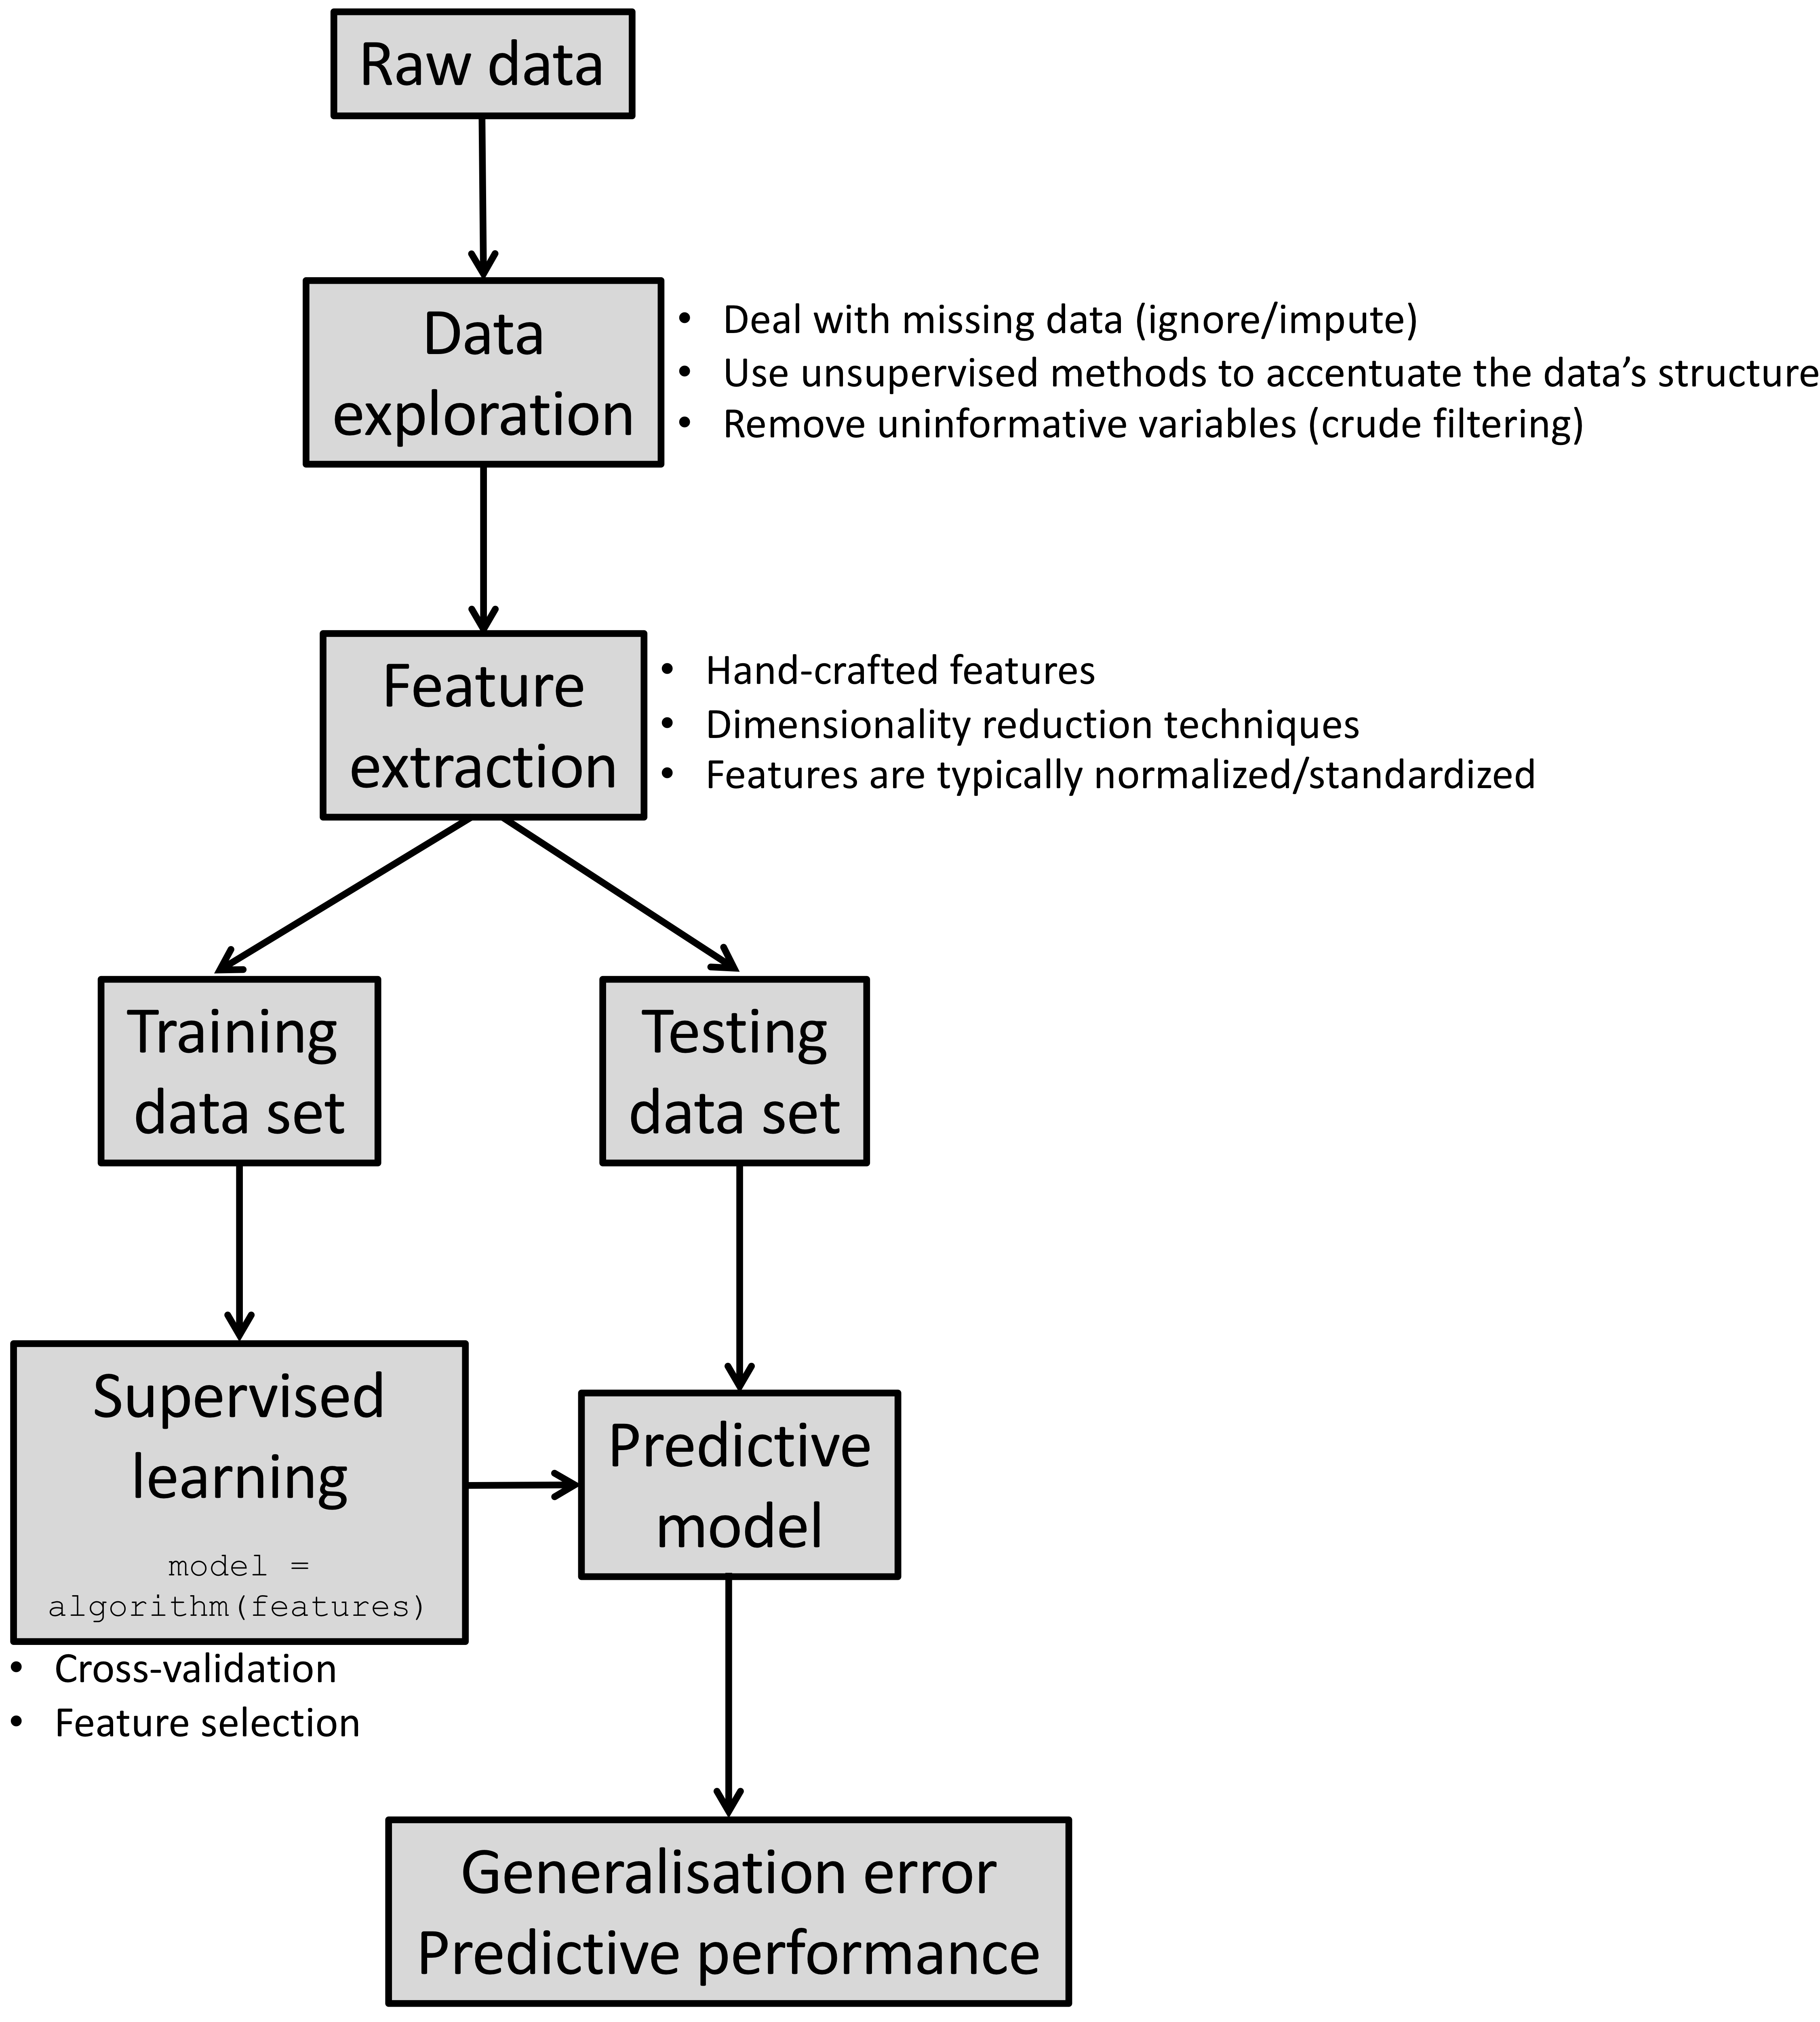
\includegraphics[width=750px]{_img//01-birdview} \end{center}

\textbf{Health warning}: Real-life data is very messy. You \emph{will} end up spending most of your time preparing your data
into a format amenable for exploration/modelling. Do not despair, in this workshop you will be provided with clean data sets
that can be used straightaway. Nevertheless, if you have not attended a course on data wrangling
and visualisation yet, I would strongly recommend doing TJ McKinley's \href{https://exeter-data-analytics.github.io/AdVis/}{course}.

\begin{comment}

\newgeometry{margin=0.5in}

# (APPENDIX) Appendix {-}

# Answers



\end{comment}


\end{document}
